\documentclass[12pt]{beamer}
%\documentclass[20pt,handout]{beamer}
\usetheme{Darmstadt}
\usepackage{graphicx}
%\usepackage[german]{babel}
\usepackage{ngerman}
\usepackage[T1]{fontenc}
\usepackage[utf8]{inputenc}
\usepackage{tikz}
\setbeamertemplate{footline}[frame number]

\newcommand{\cc}[1]{\includegraphics[height=4mm]{img/#1.png}\hspace{1mm}}
\usepackage{ifthen}
\newcommand{\license}[2][]{\\#2\ifthenelse{\equal{#1}{}}{}{\\\scriptsize\url{#1}}}
\usepackage{textcomp}
\usepackage{hyperref}

\pgfdeclareimage[height=.6cm]{c3d2logo}{./img/c3d2.pdf}


\pgfdeclarelayer{foreground}
\pgfsetlayers{main,foreground}
\logo{\pgfputat{\pgfxy(-1,0)}{\pgfbox[center,base]{\pgfuseimage{c3d2logo}}}}


\title{Smartphones und Datenschutz}
\author{\small Stephan Thamm und Stefan B"ocker\\\large Chaos Computer Club Dresden}
\date{18.03.2015}

\begin{document}
\maketitle


\section{Einleitung}
\subsection{}

\begin{frame}
    \frametitle{Chaos Computer Club}
    \begin{center}
	
\includegraphics[height=0.2\textheight]{img/chaosknoten.png}
    \end{center}	
    \begin{itemize}
      \item<1-> Verein wurde 1981 gegr"undet (\url{https://ccc.de})          
      \item<2-> Aktuell ca. 4500 Mitglieder
      \item<3-> Betreibt u.a. "Offentlichkeitsarbeit und Politikberatung      
    \end{itemize}
\end{frame}

\begin{frame}
  \frametitle{Chaos Computer Club}
  \begin{figure}
    
\includegraphics[height=0.7\textheight]{img/fingerabdruck.jpg}
  \end{figure}
\end{frame}

\begin{frame}
  \frametitle{Chaos Computer Club}
  \begin{figure}
    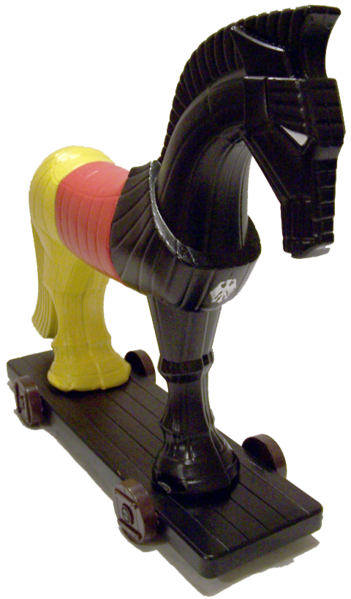
\includegraphics[height=0.7\textheight]{img/trojaner.png}
  \end{figure}
\end{frame}

\begin{frame}
    \frametitle{Chaos Computer Club}
    \begin{center}
	
\includegraphics[height=0.1\textheight]{img/c3d2_logo.png}
    \end{center}
    \begin{itemize}
      \item<1-> Chaos Computer Club Dresden (\url{https://c3d2.de})          
      \item<2-> Datenspuren: September 2015 (\url{https://datenspuren.de})
      \item<3-> Podcasts (\url{https://c3d2.de/radio.html})
      \item<4-> Chaos macht Schule (\url{https://c3d2.de/schule.html})
    \end{itemize}
\end{frame}

\section{Fragerunde}
\subsection{}

\begin{frame}
    \frametitle{Fragerunde}
    \begin{itemize}
	    \item Wieviele von ihnen nutzen aktive ein Smartphone?
	    \item Wie viele ihrer Schüler nutzen aktiv ein Smartphone?
	    \item Wie viele ihrer Schüler sind mit den Einstellmöglichkeiten ihres Smartphones vertraut?
	    \item Wie viele von ihnen sind mit den Einstellmöglichkeiten ihres Smartphones vertraut?
    \end{itemize}
\end{frame}

\section{Ebenen beim Smartphone}
\subsection{Hardware}
\begin{frame}
	\frametitle{Hardware}
	\begin{itemize}
		\item WLAN
		\item GPS
		\item Bewegungssensoren
		\item Kamera, Mikrofon
		\item Telefoniefunktion
		\item Erweiterungsslots
	\end{itemize}
\end{frame}

\subsection{Betriebssystem}
\begin{frame}
	\frametitle{Betriebssystem}
	\begin{itemize}
		\item Android Konto
		\item App Stores
		\item Zugriffsrechtemanagement
		\item Updates
	\end{itemize}
\end{frame}

\subsubsection{App Stores}
\begin{frame}
	\frametitle{App Stores}
	\begin{itemize}
		\item Zugang zum App Store wird kontrolliert
		\item Hoheit darüber, welche Software installiert werden kann
		\item Datenschutz Level wird kontrolliert
		\item Updateproblem
		\item Verknüpfung mit Cloud Diensten
	\end{itemize}
\end{frame}

\subsubsection{Apps}
\begin{frame}
	\frametitle{Apps}
	\begin{itemize}
		\item Zugriff auf persönliche Daten
		\item Zugriff auf PhoneID
		\item Zugriff auf Sensoren
		\item Zugriff auf Kamera, Mikrofon
		\item Zugriff auf Netzwerk
		\item Durch Benutzung der App entstehende Privatsphärenprobleme
	\end{itemize}
\end{frame}

\section{App Permission Restrictions}
\subsection{App Permission Restrictions}
\begin{frame}
	\frametitle{App Permission Restrictions}
	\begin{itemize}
		\item Regeln Zugriffsrechte einer App
		\item Wettbewerb um Datenschutz wird nicht gefördert
		\item Wo findet man, welche Rechte eine App braucht?
	\end{itemize}
\end{frame}

\subsection{Mitmach Teil}
\begin{frame}
	\frametitle{Ratespiel}
	\begin{itemize}
		\item Behältnis mit Zetteln mit Zugriffsrechten
		\item Auf Zettel stehen Zugriffsrechte, Rückseite hat Nummer
		\item Privatsphärenverletztendes Szenario kreieren
		\item Raten, um welche App es sich gehandelt hat
		\item Sensibilisiert die Schüler, wie man ihre Privatsphäre ausspionieren kann
		\item Szenarien sollen kreativ sein
	\end{itemize}
\end{frame}

\section{Alternative App Stores}
\subsection{Alternative App Stores}
\begin{frame}
	\frametitle{Alternative App Stores}
	\begin{itemize}
		\item Entwickler haben anderen Fokus
		\item mehr Datenschutz
		\item weniger Kommerz
		\item viele Probleme mit Community gelöst
		\item Spiele, Sensoren auslesen, \ldots
	\end{itemize}
\end{frame}
\subsection{Alternative Android ROMs}
\begin{frame}
	\frametitle{Alternative Android ROMs}
	\begin{itemize}
		\item basiert auf quelloffenen Teilen von Android
		\item meistens fügen Hersteller weitere Software hinzu
		\item alternative ROMs auf Datenschutz fixiert als "`Verkaufsargument"'
		\item Telefon muss gerootet werden, Wissen, Garantie
	\end{itemize}
\end{frame}

\begin{frame}
	\frametitle{Liste an Android ROMs, anderen OS}
	\begin{itemize}
		\item Cyanogenmod, \ldots
		\item Firefox OS
		\item Sailfish OS/Jolla
		\item Ubuntu
	\end{itemize}
\end{frame}
\end{document}
